\title{\papertitle}

\author{Rocco Schulz and Robert Wawrzyniak}
	
\publishers{Corporate State University\\Baden-Wuerttemberg - Stuttgart}

\date{
\vspace{0.6cm}
provided on 6 May 2013\\
\vspace{0.6cm}
School of: Business\\
\vspace{0.6cm}
Program: International Business Information Management\\
\vspace{0.6cm}
Course: WWI2010I\\
\vspace{0.6cm}
}





% DOCUMENT
\renewcommand{\baselinestretch}{1.5}\normalsize
\begin{document}
\pagestyle{scrheadings}

% roman numerals
\renewcommand{\thepage}{\Roman{page}}
% page numbers centered on top:
\chead{\pagemark}
\cfoot{}

%----------------------------------------------------------------------------
% Title Page
%----------------------------------------------------------------------------

% no page numbering
\thispagestyle{empty}
% include title page
\begin{titlepage}
%\vspace*{\fill}
\begin{center}
\vspace{3mm}

\textbf{\textsc{\Large 	\papertitle}} \\
\vspace{1.5cm}

\papertype \\ % Type of paper (defined in header.tex)
\vspace{0.4cm}

provided on \today \\ % Date of provision
\vspace{0.4cm}

School of: Business  \\
\vspace{0.4cm}

Program: International Business Information Management \\ % Program (defined in header.tex)
\vspace{0.4cm}

Course: WWI2010I \\ % Course (defined in header.tex)
\vspace{1.5cm}

by \\
\paperauthor % Author (defined in header.tex)
\vspace{1cm}
							
Baden-Wuerttemberg Cooperative State University Stuttgart	\\


% Note of confidentiality is only included when `confidential` is set
% to `true` in header.tex
%\textbf{Confidential}\\%
%The content of the paper must not be made available to third parties without approval of the training company.\\


\end{center}
\vspace*{\fill}
\end{titlepage}


%  \begin{abstract}
%  \vspace{1.6cm}
% % \textbf{\abstractname}: 
%  \end{abstract}


%----------------------------------------------------------------------------
% Table of Contents
%----------------------------------------------------------------------------
\renewcommand{\baselinestretch}{1.4}\normalsize
\tableofcontents
\renewcommand{\baselinestretch}{1.5}\normalsize
\newpage


%----------------------------------------------------------------------------
% Abbreviations
%----------------------------------------------------------------------------
% List needs to be indexed after each change.
% This is done by executing the following command:
% ~$ makeindex [filename].nlo -s nomencl.ist -o [filename].nls
\printnomenclature
\addcontentsline{toc}{section}{List of Abbreviations}
\nomenclature{CV}{Computer Vision}


\newpage

%----------------------------------------------------------------------------
% List Of Tables
%----------------------------------------------------------------------------
\listoftables
\addcontentsline{toc}{section}{\listtablename}
\newpage


%----------------------------------------------------------------------------
% List of Listings
%----------------------------------------------------------------------------
%\lstlistoflistings
\listoflistings
\addcontentsline{toc}{section}{List of Listings}
\newpage

% Arabic numerals for page numbering
\renewcommand{\thepage}{\arabic{page}}

% Set page number to 1: 
\setcounter{page}{1} 


%----------------------------------------------------------------------------
% Intro
%----------------------------------------------------------------------------
\section{Introduction}
\label{sec:introduction}




\subsection{Objectives}
\label{sec:objectives}



\subsection{Methodology and Structure}
\label{sec:methodology}



%----------------------------------------------------------------------------
% Theoretical Foundation
%----------------------------------------------------------------------------
\newpage
\section{RoboCup \label{sec:robo}}
Robots play soccer.
Environment is dynamic.

Long Term Goal “By mid-21st century, a team of fully autonomous humanoid robot
soccer players shall win the soccer game, comply with the official rule of the
FIFA, against the winner of the most recent World
Cup.”\footcite[Cf.][]{robo_objectives}

Computational challenges are in the environment of the RoboCup.
Comparison to chess, where computers are superior already:

\begin{table}[htbp]
\centering
\begin{savenotes}
\begin{tabular*}{0.7\textwidth}{p{0.25\textwidth} p{0.2\textwidth} p{0.2\textwidth}}
\toprule
                    &\textbf{Chess} & \textbf{Robocup} \\
\midrule 
Environment         & static		& dynamic \\
State change        & turn taking   & real time \\
Info. accessibility & complete      & incomplete \\
Sensor readings     & symbolic      & non-symbolic \\
Control             & central       & distributed \\
\bottomrule 
\end{tabular*}
  \caption[Comparison of Chess and Robocup]{Comparison of Chess and Robocup\footcite[][]{robo_objectives}}
  \label{tab:chess_comparison}
\end{savenotes}
\end{table}

\subsection{RoboCup Leagues \label{sec:robo-leagues}}

%TODO: add short description for each league

\paragraph{Humanoid}
In the Humanoid League autonomous robots with human-like bodies play soccer
against each other.
Robots may only use sensors that cover human senses to perceive their
environment. Additional technical challenges in this league are proper running and ball
kicking while keeping the balance. Robots need to localize theirselves on the
field using the available sensors.
There are three categories within the humanoid league: KidSize (30-60cm height),
TeenSize (100-120cm) and AdultSize (130cm and taller).\footcite[Cf.][]{robo_humanoid_wiki}
 
\paragraph{Middle Size}
In the Middle Size League autonomous robots with zylindric bodies of no more
than 50cm diameter play soccer in teams of up to 6 players. Robots may use
wireless networking to communicate and all sensors are deployed on-board.\footcite[Cf.][]{robo_ms}
 
\paragraph{Simulation}
\begin{quote}
In the 2D Simulation League, two teams of eleven autonomous software programs
(called agents) each play soccer in a two-dimensional virtual soccer stadium
represented by a central server, called SoccerServer.\footcite[][]{robo_simu_wiki}

\end{quote}
Agents receive relative and noisy input from their virtual sensors which they can use to
calculate and perform desired actions. There is also a 3D Simulation League which differs
from the 2D League by adding a third dimension and more complex physical
models.\footcite[Cf.][]{robo_simu_wiki}
 
\paragraph{Small Size}
In the Small Size League teams of five robots each compete on a field of 5.05m~x 4.05m.
Robots must fit in a circle with a diameter of 18cm and must not be higher than 15cm.
Robots are not fully autonomous as they can be controlled by off-field computers which receive
game information via a central software server which tracks locations and other parameters
of the game.\footcite[Cf.][]{robo_ssl_wiki}
This software is called SSL-Vision and will be covered in further detail in section
\ref{sec:ssl-vision}.
 
\paragraph{Standard Platform}
In the Standard Platform League all teams compete with identical
robots.\footcite[Cf.][]{robo_std_wiki}
\begin{quotation}
The robots operate fully autonomously,
i.e. there is no external control, neither by humans nor by computers. The
current standard platform used is the humanoid NAO by Aldebaran
Robotics.\footcite[][]{robo_std_wiki}
\end{quotation}

\subsection{Related Research Areas \label{sec:robo-research}}
Various research areas are relevant for the further development of the RoboCup
and the capabilities of the robots used in the matches. An overview of the most
important research areas is given in the list below:\footcite[Cf.][]{robo_objectives}
\begin{itemize}
  \item real-time sensor fusion
  \item reactive behavior
  \item strategy acquisition
  \item learning
  \item real-time planning
  \item multi-agent systems
  \item context recognition
  \item computer vision
  \item strategic decision-making
  \item motor control
  \item intelligent robot control
\end{itemize}

The main role of computer vision is the detection of game objects and object
localization on the field and will be described in further detail in the next
section.

\newpage
\section{Computer Vision at RoboCup \label{sec:cv-robo}}

Computer vision is used in all leagues of the RoboCup.
The leagues can be categorized in fully autonomously (distributed) and centrally
controlled robots. The Small Size League fits into the latter of these two categories.

\subsection{Centralized}
In the Small Size League a centralized computer vision system captures images
of the game and pre-processes them before broadcasting the information to the teams
for further processing.

Robots and the ball are tracked via markings. A camera above the field sends
data to a computer which does real time analysis of image data to determine
positions and directions using COMPUTER VISION

\begin{quote}
All objects on the field are tracked by a standardized vision system that
processes the data provided by two cameras that are attached to a camera bar
located 4m above the playing surface. The vision system - called SSL-Vision - is
an open source project maintained by the league's community.\footcite[Cf.][]{robo_ssl_wiki}
\end{quote}

Robots and the ball are tracked via markings. A camera above the field sends
data to a computer which does real time analysis of image data to determine
positions and directions using COMPUTER VISION

\begin{savenotes}
\begin{figure}[htbp]
\begin{center}
  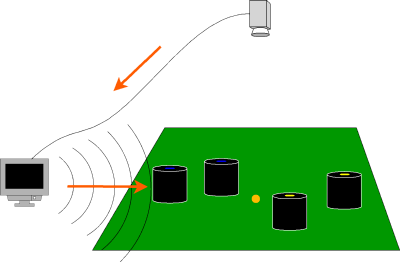
\includegraphics[width=0.6\textwidth]{img/ssl_dataflow.png}
  \caption[Data flow in SSL camera setup]{Data flow in SSL camera setup\footcite[][]{robo_ssl_wiki}}
  \label{fig:ssl_dataflow}
\end{center}
\end{figure}
\end{savenotes}

\subsection{Distributed / Autonomous}
for other leagues. each robot has own cv.
In most other leagues robots have to rely on their own sensing, however they may
communicate with each other over the air.
Less computation power available, CV data needs to be translated to position,
etc. Robots need to keep track of other players and the ball + movements and
velocity of objects.



\newpage
\section{SSL-Vision \label{sec:ssl-vision}}


\subsection{Application Overview \label{sec:ssl-overview}}
SSL-Vision is the open source software which is used in the Small Size League to
track game objects on the field. It is written in C++ and uses multiple threads
for best performance. The software comes with a graphical user interface (GUI)
which can be used for configuration and monitoring of input and output data.

The software has a multi-camera stack where one thread is assigned for each camera.
For each camera plugins can be enabled to perform various image processing
tasks. These plugins can operate together by using common interfaces for data
transfer.

SSL-Vision receives raw video streams from various cameras as input. The
computed information, such as robots identified by id and their appropriate
coordinates on the field are broadcasted to the teams' servers for further
processing and decision making. For testing and development purposes it is also
possible to use filestreams as input for the system.

\subsection{The Image Processing Flow}
The processing stack for the Small Size League domain follows a multi-stage
approach which is described in this section.\\
SSL-Vision relies on colored markers to identify robots on the field.
Each robot on the field is uniquely identifiable by a colored marker that
consists of a combination for team identification as well as additional color
elements to provide uniqueness for each robot.\footcite[Cf.][5]{zickler_ssl_vision}
SSL-Vision needs to determine robots' real-world locations (as opposed to the
location in the image), directions and IDs.
In order to get these information different algorithms and techniques need to be
applied in real time. One of these is color segmentation, which serves as a 
base for the pattern detection step in the overall processing flow.


\subsubsection{Color Segmentation}
Color segmentation is done with plugins for color thresholding, runlength-encoding,
region extraction and region sorting.\footcite[Cf.][]{zickler_ssl_vision}

\paragraph{Color thresholding}
Color thresholding is done via a lookup table which maps from the input image's
3d color space (YUV) to a unique color label which represents any of the marker
colors, the ball color or other desired colors.\footcite[Cf.][p. 4 et sq.]{zickler_ssl_vision}
The plugin uses YUV for the color space mapping, which is for instance used
in PAL and NTSC videos. The \textit{Y} in YUV represents lumination and
\textit{U/V} is used for the color representation.

\begin{savenotes}
\begin{figure}
        \centering
        \begin{subfigure}[b]{0.3\textwidth}
                \centering
                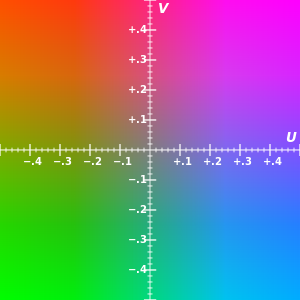
\includegraphics[width=\textwidth]{img/YUV.png}
                \caption[YUV colorspace]{YUV colorspace\footcite[][]{yuv_img}}
                \label{fig:yuv_normal}
        \end{subfigure}%
        ~ %add desired spacing between images, e. g. ~, \quad, \qquad etc.
          %(or a blank line to force the subfigure onto a new line)
        \begin{subfigure}[b]{0.3\textwidth}
                \centering
                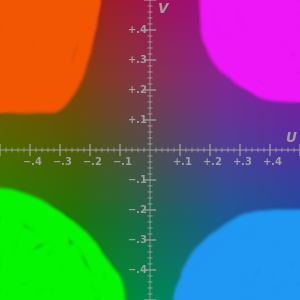
\includegraphics[width=\textwidth]{img/YUV_LUT.png}
                \caption{Mapped YUV colorspace}
                \label{fig:yuv_mapped}
        \end{subfigure}

        \caption{Exemplary YUV colorspace mapping}\label{fig:yuv}
\end{figure}
\end{savenotes}

Fig. \ref{fig:yuv} illustrates how the color mapping works. Fig.
\ref{fig:yuv_normal} shows the normal YUV colorspace and Fig.
\ref{fig:yuv_mapped} shows the mapped colorspace which replaces regions in the
colorspace with a single color value. The colors in the input images are
replaced acordingly to the color mappings before further processing by the other
plugins takes place.


\paragraph{Runlength encoding}

Runlength encoding is a simple compression technique in image processing. The
idea behind this technique is to represent recurring pixel values with a number
rather than storing each pixel value. Due to the previously applied color thresholding
this compression technique is very effective.
The algorithm for the runlength encoding iterate through all rows of the picture
and for each row it compares the current pixel with the previous pixel. When the pixel values are
equal they are merged (i.e. stored as one unit). This is repeated for all pixels within each row.
The line by line runlength encoding is applied on the thresholded image to speed up the
region extraction that follows.
The source code of the runlength encode plugin is available in the SSL-Vision code 
repository.\footnote{See \url{http://code.google.com/p/ssl-vision/source/browse/trunk/src/app/plugins/plugin_runlength_encode.cpp}}

\paragraph{Region extraction}
After the runlength encoding pixels are connected horizontally, however they
need to be connected vertically as well to retrieve regions.\\
The region extraction plugin uses a tree-based union find algorithm to traverse the
runlength-encoded image and merge neighboring runs of similar colors.\footcite[Cf.][p. 6 et sq.]{zickler_ssl_vision}

The underlying data structure of the union find algorithm is a reverse tree, where each node points to its parent node.
The root note points to itself.\footcite[Cf.][]{wa_union_find}
Each set of elements is represented in such a tree.\\
The algorithm basically consists of two elementary methods: A \textit{union}-method and a \textit{find}-method.
The find method returns the root node for any given node. This is implemented by following the parent-pointers
until the root node has been found. The union-method merges any two sets by hanging the root node of one set to the
root node of the other set.\footcite[Cf.][]{wa_union_find}

Thanks to the flat tree structures it is computationally cheap to find root nodes and to join multiple sets of pixels
to larger sets.\\
Bounding boxes and centroids of all merged regions are computed after the merging and finally
sorted by color and size. The centroids are later used for location determination.

The implementation of the algorithm is located in
\texttt{cmvision\_region.cpp}.\footnote{See
\url{http://code.google.com/p/ssl-vision/source/browse/trunk/src/shared/cmvision/cmvision_region.cpp\#97}}




\subsubsection{Pattern Detection}
After the extraction of regions and computation of their real-world coordinates,
the processing continues with the pattern detection plugin.
This plugin extracts the identities, locations and orientations of robots on the field.
Additionally the location of the ball is determined.\footcite[Cf.][p. 6 et sq.]{zickler_ssl_vision}
The internal detection algorithm
is described in detail in a publication by \citeauthor{bruce_2003}.\footcite[Cf.][]{bruce_2003}

%----------------------------------------------------------------------------
% Closing
%----------------------------------------------------------------------------

\clearpage
\section{Conclusion and Outlook}
\label{sec:conclusion}
SSL Vision is pretty mature.



%----------------------------------------------------------------------------
% APPENDIX
%----------------------------------------------------------------------------
% Appendix sections need to be within the subappendices environment.
% Use the command \appsection{title} instead of \section to introduce each
% appendix. This will add each appendix to the list of appendices.

% sets the appendix environment and resets the section counters
\newpage \begin{appendices} 
\appendixtocon %adds an 'Appendices' entry to the toc

\appendixpage %prints the title on the page

\subsection*{\listappendixname}
%--------------------------------
% style of the \listofappendices command is defined in header.tex
\listofappendices

% begin appendices on a new page
\newpage

%start environment for subappendices, so that new sections are formatted as
%subsections of appendix
\begin{subappendices}
\renewcommand{\setthesubsection}{\arabic{subsection}:}%

\appsection{Source Code}
\label{apx:code-template}


% close the appendices environment
\end{subappendices}
\end{appendices}
